% !TeX spellcheck = en_US
% !TeX root = ./0_article.tex

\section{Validating and completing the models}
With the aim of verifying the soundness of the previous conclusions, we set up experiments using an actual IC composed of both triple-well and dual-well substrate on a monolithic die.
These experiments consist in verifying if the difference in injected energy depending on the substrate type is actually significant or not.

The target used is a STM32F439 microcontroller, alongside the platform presented in the first chapter.
We call these experiments "IC ground current mapping", and quite naturally, they consist in measuring in specific conditions the current at the target circuit external ground connection.
The entirety of the IC is mapped, and a voltage pulse is injected at each location.
Then, we measure the current at the circuit ground and calculate its RMS value to represent it into a two-dimensional cartography.
% !TeX spellcheck = en_US
% !TeX root = ./0_article.tex

\begin{figure}[h]
	\centering
	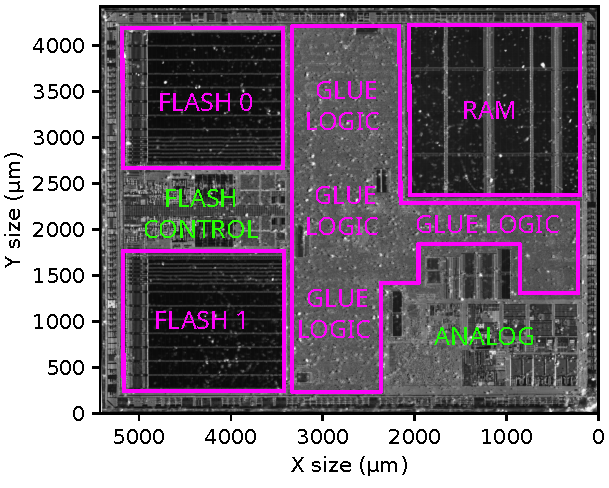
\includegraphics[width=\columnwidth]{./figures/stmPhotoImshow.pdf}
	\caption{Caption}
	\label{stm_ir_photo}
\end{figure}

Knowing the coarse structure of the considered IC, in addition to having insights on the substrate type, we could draw the coarse structure picture shown in Fig. \ref{stm_ir_photo}.
The "glue logic" regions are known to be made with triple-well substrates, while the "flash control" and "analog" regions are made with dual-well substrates.
\textcolor{orange}{The memories, however, are made of a mix of both.}
